\documentclass[aspectratio=169]{beamer}
\usepackage[utf8]{inputenc}
\usepackage[T1]{fontenc}
\usepackage{lmodern}
\usepackage{graphicx}
\usepackage{tikz}
\usepackage{listings}
\usepackage{xcolor}
\usepackage{fontawesome5}

% Theme and color scheme
\usetheme{Madrid}
\usecolortheme{default}

% Custom colors
\definecolor{primaryblue}{RGB}{44,82,130}
\definecolor{lightblue}{RGB}{66,153,225}
\definecolor{darkgray}{RGB}{45,55,72}
\definecolor{lightgray}{RGB}{247,250,252}

% Set theme colors
\setbeamercolor{structure}{fg=primaryblue}
\setbeamercolor{frametitle}{bg=primaryblue,fg=white}
\setbeamercolor{title}{fg=primaryblue}
\setbeamercolor{block title}{bg=lightblue,fg=white}
\setbeamercolor{block body}{bg=lightgray}

% Custom title page
\setbeamertemplate{title page}{
  \begin{tikzpicture}[remember picture,overlay]
    \fill[primaryblue] (current page.north west) rectangle ([yshift=-3cm]current page.north east);
    \fill[lightblue] ([yshift=-3cm]current page.north west) rectangle ([yshift=-3.2cm]current page.north east);
  \end{tikzpicture}
  
  \vspace{1cm}
  \begin{center}
    {\Huge\color{white}\textbf{Inventory Management System}}\\[0.5cm]
    {\Large\color{white}Complete Technical \& Deployment Guide}\\[1.5cm]
    
    \begin{beamercolorbox}[wd=0.8\textwidth,center,rounded=true,shadow=true]{block body}
      \vspace{0.3cm}
      {\large\textbf{Prepared for:}}\\[0.2cm]
      {\Large\color{primaryblue}\textbf{Marquardt India Pvt. Ltd.}}\\[0.5cm]
      {\large\textbf{MQI Internship Team (2025)}}\\[0.3cm]
    \end{beamercolorbox}
    
    \vspace{1cm}
    \begin{beamercolorbox}[wd=0.6\textwidth,center,rounded=true]{block title}
      \vspace{0.2cm}
      {\textbf{Development Team}}\\[0.3cm]
      Meghana Prathipati\\
      Neha Gaikwad\\
      Priyanshu Kumar Sharma\\[0.2cm]
    \end{beamercolorbox}
  \end{center}
}

% Code listing style
\lstset{
  backgroundcolor=\color{lightgray},
  basicstyle=\ttfamily\small,
  keywordstyle=\color{primaryblue}\bfseries,
  commentstyle=\color{darkgray}\itshape,
  frame=single,
  breaklines=true,
  showstringspaces=false
}

% Document information
\title{Inventory Management System}
\subtitle{Complete Technical \& Deployment Guide}
\author{Meghana Prathipati \and Neha Gaikwad \and Priyanshu Kumar Sharma}
\institute{MQI Internship Team (2025)}
\date{\today}

\begin{document}

% Title slide
\begin{frame}[plain]
  \titlepage
\end{frame}

% Slide 2: Executive Overview
\begin{frame}{Executive Overview}
  \begin{block}{Document Purpose}
    \begin{itemize}
      \item Comprehensive installation, configuration, and deployment manual
      \item Designed for developers, system administrators, and IT operations staff
      \item Covers migration, installation, and operation across various environments
    \end{itemize}
  \end{block}
  
  \begin{block}{Target Environments}
    \begin{itemize}
      \item Local development setup (Windows/Linux with MySQL)
      \item Windows Service for enterprise environments
      \item Google Cloud Platform with App Engine and Cloud SQL
      \item Docker containers for consistent deployments
    \end{itemize}
  \end{block}
\end{frame}

% Slide 3: System Overview
\begin{frame}{System Overview}
  \begin{center}
    {\Large\textbf{Marquardt Inventory \& Asset Management System (MIAMS)}}
  \end{center}
  
  \begin{columns}[T]
    \begin{column}{0.48\textwidth}
      \begin{block}{Role-Based Access}
        Separate interfaces for Employees, Monitors, and Administrators
      \end{block}
      
      \begin{block}{Automated Workflows}
        Email notifications, approval processes, audit logging
      \end{block}
    \end{column}
    
    \begin{column}{0.48\textwidth}
      \begin{block}{Real-Time Management}
        Live tracking of product availability and assignments
      \end{block}
      
      \begin{block}{AI-Powered Assistant}
        Intelligent chatbot for real-time system queries
      \end{block}
    \end{column}
  \end{columns}
\end{frame}

% Slide 4: System Architecture
\begin{frame}{System Architecture}
  \begin{center}
    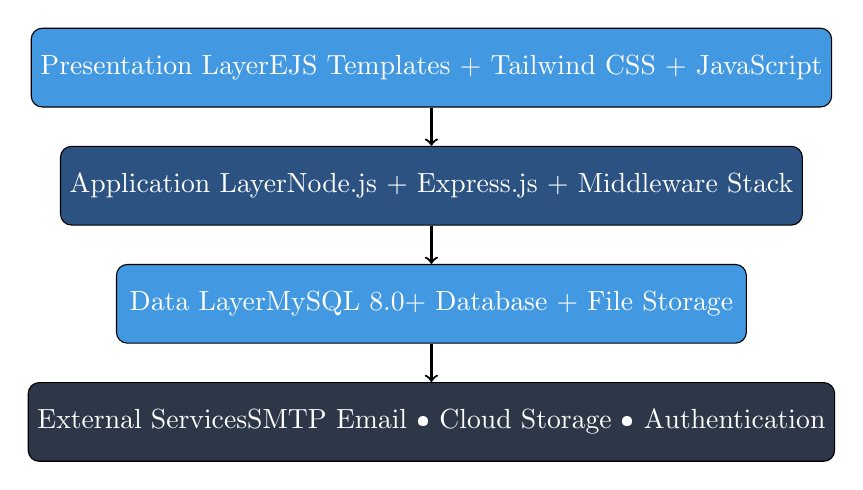
\begin{tikzpicture}[node distance=1.5cm]
      \node[draw, fill=lightblue, text=white, rounded corners, minimum width=8cm, minimum height=1cm] (presentation) {Presentation Layer\\EJS Templates + Tailwind CSS + JavaScript};
      
      \node[draw, fill=primaryblue, text=white, rounded corners, minimum width=8cm, minimum height=1cm, below of=presentation] (application) {Application Layer\\Node.js + Express.js + Middleware Stack};
      
      \node[draw, fill=lightblue, text=white, rounded corners, minimum width=8cm, minimum height=1cm, below of=application] (data) {Data Layer\\MySQL 8.0+ Database + File Storage};
      
      \node[draw, fill=darkgray, text=white, rounded corners, minimum width=8cm, minimum height=1cm, below of=data] (external) {External Services\\SMTP Email • Cloud Storage • Authentication};
      
      \draw[->, thick] (presentation) -- (application);
      \draw[->, thick] (application) -- (data);
      \draw[->, thick] (data) -- (external);
    \end{tikzpicture}
  \end{center}
\end{frame}

% Slide 5: Technology Stack
\begin{frame}{Technology Stack}
  \begin{columns}[T]
    \begin{column}{0.48\textwidth}
      \begin{block}{Frontend}
        HTML5, Tailwind CSS, EJS templates
      \end{block}
      
      \begin{block}{Database}
        MySQL 8.0+ (Google Cloud SQL for production)
      \end{block}
      
      \begin{block}{CI/CD}
        GitHub Actions (test, lint, deploy)
      \end{block}
    \end{column}
    
    \begin{column}{0.48\textwidth}
      \begin{block}{Backend}
        Node.js 20+, Express.js, middleware packages
      \end{block}
      
      \begin{block}{Authentication}
        bcryptjs hashing, express-session management
      \end{block}
      
      \begin{block}{Deployment}
        Windows Service, Google App Engine, Docker
      \end{block}
    \end{column}
  \end{columns}
\end{frame}

% Slide 6: System Requirements
\begin{frame}{System Requirements}
  \begin{block}{Hardware Requirements}
    \begin{itemize}
      \item OS: Windows 10+ / Windows Server 2016+ / Linux
      \item RAM: 4GB+ recommended (8GB for production)
      \item Disk: 1GB free space (SSD recommended)
      \item Network: Ethernet for LAN access
      \item Administrative privileges on target machine
    \end{itemize}
  \end{block}
  
  \begin{block}{Software Prerequisites}
    \begin{itemize}
      \item Node.js v20 or higher
      \item MySQL Server 8.0+
      \item Git (optional for development)
      \item Docker Desktop (optional for containerization)
    \end{itemize}
  \end{block}
\end{frame}

% Slide 7: Installation Process
\begin{frame}[fragile]{Installation Process}
  \begin{block}{Step 1: Obtain Project}
    \begin{lstlisting}[language=bash]
git clone https://github.com/Interns-MQI-25/project-interns.git
cd project-interns
npm install
    \end{lstlisting}
  \end{block}
  
  \begin{block}{Step 2: Database Setup}
    \begin{lstlisting}[language=bash]
mysql -u root -p
CREATE DATABASE product_management_system;
SOURCE sql/database.sql;
    \end{lstlisting}
  \end{block}
\end{frame}

% Slide 8: Deployment Options
\begin{frame}{Deployment Options}
  \begin{columns}[T]
    \begin{column}{0.48\textwidth}
      \begin{block}{Windows Service}
        Enterprise deployment with automatic startup
        \begin{itemize}
          \item \texttt{cd deployment}
          \item \texttt{install-service.bat}
        \end{itemize}
      \end{block}
      
      \begin{block}{Google Cloud Platform}
        Production scalable deployment
        \begin{itemize}
          \item \texttt{gcloud app deploy}
          \item \texttt{app.yaml --quiet}
        \end{itemize}
      \end{block}
    \end{column}
    
    \begin{column}{0.48\textwidth}
      \begin{block}{Manual Node Start}
        Development and debugging
        \begin{itemize}
          \item \texttt{node server.js}
          \item \texttt{npm run dev}
        \end{itemize}
      \end{block}
      
      \begin{block}{Docker Container}
        Consistent containerized deployment
        \begin{itemize}
          \item \texttt{docker pull priyanshuksharma/}
          \item \texttt{project-interns:latest}
        \end{itemize}
      \end{block}
    \end{column}
  \end{columns}
\end{frame}

% Slide 9: Security Architecture
\begin{frame}{Security Architecture}
  \begin{block}{Authentication \& Authorization}
    \begin{itemize}
      \item bcrypt password hashing with configurable salt rounds
      \item Secure session cookies with HttpOnly and Secure flags
      \item Three-tier role-based access (Employee, Monitor, Administrator)
      \item CSRF protection with token validation
    \end{itemize}
  \end{block}
  
  \begin{block}{Data Protection}
    \begin{itemize}
      \item HTTPS/TLS for all client-server communication
      \item Database encryption for sensitive data storage
      \item XSS prevention through proper output encoding
      \item File upload security with type validation and size limits
    \end{itemize}
  \end{block}
\end{frame}

% Slide 10: Database Architecture
\begin{frame}{Database Architecture}
  \begin{block}{Core Tables}
    \begin{itemize}
      \item \textbf{users} - User accounts and authentication
      \item \textbf{employees} - Employee details and department mapping
      \item \textbf{products} - Product catalog and inventory
      \item \textbf{product\_requests} - Employee product requests
      \item \textbf{product\_assignments} - Approved product assignments
      \item \textbf{product\_attachments} - File attachments for products
    \end{itemize}
  \end{block}
  
  \begin{block}{Database Features}
    \begin{itemize}
      \item MySQL 8.0+ with InnoDB storage engine for ACID compliance
      \item Connection pooling with automatic reconnection
      \item Normalized structure with foreign key constraints
    \end{itemize}
  \end{block}
\end{frame}

% Slide 11: Monitoring & Maintenance
\begin{frame}[fragile]{Monitoring \& Maintenance}
  \begin{block}{System Monitoring}
    \begin{itemize}
      \item Real-time health checks and status monitoring
      \item Application logs in daemon folder
      \item Google Cloud logging for production deployment
    \end{itemize}
  \end{block}
  
  \begin{block}{Backup Strategy}
    \begin{lstlisting}[language=bash]
# Database backup
mysqldump -u sigma -psigma product_management_system > backup.sql

# File system backup
tar -czf uploads_backup.tar.gz uploads/
    \end{lstlisting}
  \end{block}
\end{frame}

% Slide 12: Troubleshooting
\begin{frame}[fragile]{Troubleshooting}
  \begin{block}{Common Issues}
    \begin{itemize}
      \item \textbf{Service won't start:} Check daemon/*.err.log and Windows Event Viewer
      \item \textbf{Port 3000 in use:} netstat -ano | findstr :3000, then kill process
      \item \textbf{DB connection errors:} Verify .env settings and MySQL service status
      \item \textbf{Authentication issues:} Visit /setup endpoint to create admin users
    \end{itemize}
  \end{block}
  
  \begin{block}{Debug Commands}
    \begin{lstlisting}[language=bash]
# Check service status
sc query "marquardtinventorymanagement.exe"

# View logs
gcloud app logs tail -s default
    \end{lstlisting}
  \end{block}
\end{frame}

% Slide 13: Google Cloud Deployment
\begin{frame}[fragile]{Google Cloud Platform Deployment}
  \begin{block}{Cloud SQL Setup}
    \begin{lstlisting}[language=bash]
gcloud sql instances create product-management-db \
  --database-version=MYSQL_8_0 \
  --tier=db-f1-micro \
  --region=us-central1
    \end{lstlisting}
  \end{block}
  
  \begin{block}{App Engine Configuration}
    \begin{itemize}
      \item Runtime: Node.js 20
      \item Cloud SQL integration with socket path
      \item Automatic scaling (1-2 instances)
      \item Environment-specific database configuration
    \end{itemize}
  \end{block}
  
  \begin{block}{Post-Deployment}
    \begin{itemize}
      \item Visit /setup endpoint to create admin users
      \item Change default passwords immediately
      \item Test all functionality
    \end{itemize}
  \end{block}
\end{frame}

% Slide 14: Key Features
\begin{frame}{Key Features \& Capabilities}
  \begin{columns}[T]
    \begin{column}{0.48\textwidth}
      \begin{block}{Core Functionality}
        \begin{itemize}
          \item Product catalog management
          \item Employee request workflows
          \item Real-time inventory tracking
          \item Automated email notifications
          \item Comprehensive audit logging
        \end{itemize}
      \end{block}
    \end{column}
    
    \begin{column}{0.48\textwidth}
      \begin{block}{Advanced Features}
        \begin{itemize}
          \item AI-powered chatbot with NLP
          \item Real-time database queries
          \item Role-based dashboards
          \item Mobile-responsive design
          \item Gmail SMTP integration
        \end{itemize}
      \end{block}
    \end{column}
  \end{columns}
\end{frame}

% Slide 15: Conclusion
\begin{frame}{Conclusion \& Next Steps}
  \begin{block}{Key Achievements}
    \begin{itemize}
      \item Comprehensive inventory management system with role-based access
      \item Modern web architecture with scalable cloud deployment
      \item Advanced security features and audit logging
      \item AI-powered assistant for real-time system queries
      \item Multiple deployment options for different environments
    \end{itemize}
  \end{block}
  
  \begin{block}{Next Steps}
    \begin{itemize}
      \item Deploy to production environment
      \item Configure monitoring and alerting
      \item Train users on system functionality
      \item Implement regular backup procedures
    \end{itemize}
  \end{block}
  
  \begin{block}{Support Resources}
    \begin{itemize}
      \item GitHub: github.com/Interns-MQI-25/project-interns
      \item Production: mqi-ims.uc.r.appspot.com
      \item Docker Hub: priyanshuksharma/project-interns
    \end{itemize}
  \end{block}
\end{frame}

\end{document}